The alpha-beta transform, also known as the Clarke transform, is a fundamental
mathematical tool used to simplify the analysis of three-phase electric
machines. It is named after Edith Clarke, who published papers in 1937 and 1938
introducing modified calculation methods for handling unbalanced three-phase
problems~\cite{E. Clarke}.

\subsection{What is Clarke Transform?}
\begin{figure}[ht]
    \centering
    \resizebox{0.4\linewidth}{!}{
        \begin{tikzpicture}[auto, node distance=2cm, >=Latex]
            % Define the origin
            \coordinate (O) at (0,0);

            % Define the vectors
            \coordinate (A) at ({3*cos(0)},{3*sin(0)});
            \coordinate (B) at ({3*cos(120)},{3*sin(120)});
            \coordinate (C) at ({3*cos(240)},{3*sin(240)});
            \coordinate (alpha) at ({3.8*cos(0)},{3.8*sin(0)});
            \coordinate (beta) at ({3.8*cos(90)},{3.8*sin(90)});

            % Draw the main axes
            \draw[->] (O) -- (B) node[above] {$B$-axis};
            \draw[->] (O) -- (C) node[below] {$C$-axis};
            \draw[->] (O) -- (A) node[below] {$A$-axis};

            % Draw the Clarke axes
            \draw[thick, ->] (O) -- (alpha) node[below right] {$\alpha$-axis};
            \draw[thick, ->] (O) -- (beta)  node[above right] {$\beta$-axis};

            % Draw the angular velocity indication
            % \draw[->] (1,1.5) arc[start angle=60, end angle=90, radius=1.5cm];
            % \node at (1.5,2) {$\omega=0$};

        \end{tikzpicture}
    }
    \caption{Clarke Frame of reference}
    \label{fig:Clarke Frame of reference}
\end{figure}

E. Clarke developed the method for transforming stationary circuits into a
stationary reference frame. In Clarke’s transformation, the two-phase
stationary variables are represented as $\alpha$ and $\beta$, with the
$\alpha$-axis and $\beta$-axis being orthogonal to each other~\cite{DSP-Based
    Electromechanical Motion Control}.This transformation simplifies the analysis
of three-phase electrical systems by projecting the original quantities onto a
stationary reference frame. It decomposes the three-phase variables into two
orthogonal components: alpha ($\alpha$) and beta ($\beta$), which are aligned
with the stationary reference axes, called the Clarke reference frame. The
transform matrix is given by:
\begin{equation*}
    T_{\alpha\beta0} = \frac{2}{3}
    \begin{bmatrix}
        1 & -\frac{1}{2}       & -\frac{1}{2}       \\
        0 & \frac{\sqrt{3}}{2} & \frac{\sqrt{3}}{2} \\
        1 & 1                  & 1
    \end{bmatrix}
\end{equation*}


\subsection{Derivation of the Clarke Transform Matrix}

\begin{figure}[h]
    \centering
    \begin{subfigure}[b]{0.5\textwidth}
        \centering
        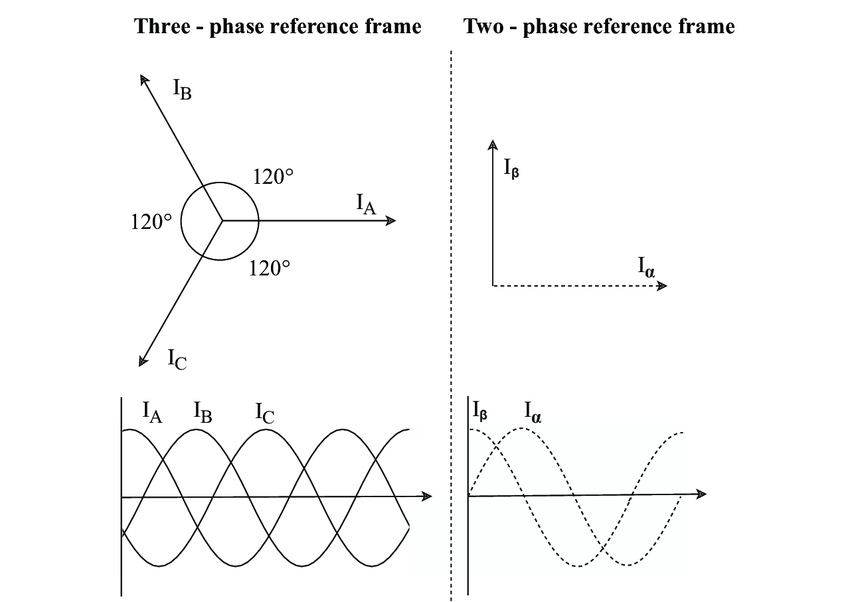
\includegraphics[width=\textwidth]{Clarke-transformation-coordinates.png}
        \caption{Clarke transformation}
        \label{fig:Clarke transformation}
    \end{subfigure}%
    \begin{subfigure}[b]{0.5\textwidth}
        \centering
        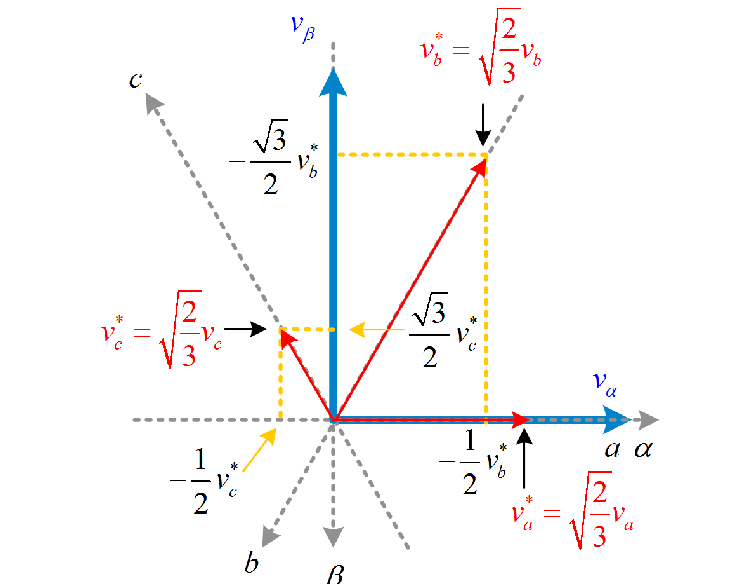
\includegraphics[width=\textwidth]{clarkederivation.png}
        \caption{Clarke transformation Derivation}
        \label{fig:Clarke transformation Derivation}
    \end{subfigure}
    \caption{Clarke transformation and its derivation}
    \label{fig:combined_Clarke}
\end{figure}


To derive the Clarke transformation, we resolve the three-phase quantities \(
V_a, V_b, V_c \) along the \(\alpha\) and \(\beta\) axes. The transformed
quantities \( V_\alpha \) and \( V_\beta \) are simplified according to Figure
\ref{fig:Clarke transformation Derivation}. The normalization term \(
\frac{2}{3} \) ensures that the magnitudes of the quantities in the Clarke
frame match those of the three-phase frame.

\begin{equation*}
    V_\alpha = \frac{2}{3}(V_a - \frac{1}{2} V_b - \frac{1}{2} V_c)
\end{equation*}
\begin{equation*}
    V_\beta = \frac{2}{3}(\frac{\sqrt{3}}{2} V_b - \frac{\sqrt{3}}{2} V_c)
\end{equation*}

\noindent
Converting this to matrix form, we get:
\begin{equation*}
    \begin{bmatrix}
        V_\alpha \\
        V_\beta  \\
        V_0
    \end{bmatrix}
    =\frac{2}{3}
    \begin{bmatrix}
        1 & -\frac{1}{2}       & -\frac{1}{2}       \\
        0 & \frac{\sqrt{3}}{2} & \frac{\sqrt{3}}{2} \\
        1 & 1                  & 1
    \end{bmatrix}
    \begin{bmatrix}
        V_a \\
        V_b \\
        V_c
    \end{bmatrix}
\end{equation*}
\noindent
or we can write it as:
\begin{equation*}
    V_{\alpha\beta0} = T_{\alpha\beta0} V_{abc}
\end{equation*}

\noindent
Where,
\begin{equation*}
    V_{\alpha\beta0} = \begin{bmatrix}
        V_\alpha \\
        V_\beta  \\
        V_0
    \end{bmatrix}
\end{equation*}
\begin{equation*}
    V_{abc} = \begin{bmatrix}
        V_a \\
        V_b \\
        V_c
    \end{bmatrix}
\end{equation*}
\begin{equation*}
    T_{\alpha\beta0} = \frac{2}{3}
    \begin{bmatrix}
        1 & -\frac{1}{2}       & -\frac{1}{2}       \\
        0 & \frac{\sqrt{3}}{2} & \frac{\sqrt{3}}{2} \\
        1 & 1                  & 1
    \end{bmatrix}
\end{equation*}

\noindent
For a balanced three-phase system where \( V_a + V_b + V_c = 0 \), the equations simplify to:
\begin{equation*}
    V_\alpha = V_a
\end{equation*}
\begin{equation*}
    V_\beta = \frac{2}{\sqrt{3}} (V_a + 2 V_b)
\end{equation*}
\begin{equation*}
    V_0 = 0
\end{equation*}